%!TEX root = ../master_thesis.tex

\chapter{Constructing dependency graphs}
\label{chapter:dependency_graph}

In this chapter we investigate how to construct a graph of application dependencies from a deployed and running microservice architecture. We first introduce the assumptions regarding the properties of the graph. Then we propose four methods for graph construction. We end the chapter by discussing and summarizing our findings.

\section{Theory}

In literature dependency graphs often are understood as ``program dependence graphs'' \cite{Horwitz} which model how a program works internally on the granularity of software modules, control flow or data flow. In this work, we use the granularity level of applications and dependencies between these as the basis for dependency graphs.

\subsubsection{Directed graph}

A \textbf{directed graph} (or ``digraph'') consists of \emph{vertices} and \emph{directed edges} \cite{ChartrandGary}. The edges connect the vertices. Every edge has a direction, leaving from one vertex and arriving at another vertex. All edges leaving from a vertex are called \emph{outgoing} edges. All edges arriving at a vertex are called \emph{incoming} edges.

\textbf{Vertices} represent applications in a microservice architecture.

Earlier in \nref{sec:software_environment_terminology} we established that one application has many processes and each process might implement or consume many services. Thus if there are many processes (or services) for one application in the graph, these would all be represented by one vertex for the application they belong to.

\textbf{Directed edges} represent service dependencies between applications.

A service dependency is the fact that a process is the consumer of a service (as explained earlier in section \ref{subsec:service_depenedency}). The direction of the directed edge follows the direction of the service dependency, from service consumer to service provider. If the vertices represent applications, the service dependency may exist for these as well, since processes and service always belong to exactly one application

\subsubsection{Example graph}

\nref{fig:digraph_example} shows a graphical example. It shows the following information:
\begin{titemize}
  \item Application A is dependent on Application B
  \item Application A is dependent on Application C
  \item Application B is dependent on Application D
\end{titemize}

\begin{figure}[h]
  \begin{center}
    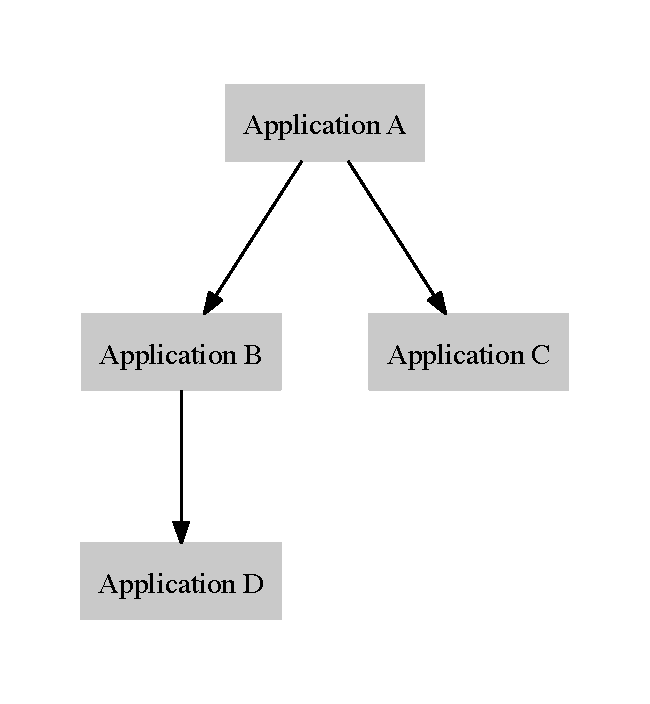
\includegraphics[width=0.48\textwidth]{images/directed-graph-example.pdf}
  \end{center}
  \caption{Dependency graph: example}
  \label{fig:digraph_example}
\end{figure}

\vfill\clearpage

\section{Methods for construction}

To construct a dependency graph from a deployed microservice architecture, we propose four methods in this chapter:
\begin{titemize}
  \item[] {\small\ref{subsec:graph_manual_annotation} \ncref{subsec:graph_manual_annotation}}
  \item[] {\small\ref{subsec:from_smi} \ncref{subsec:from_smi}}
  \item[] {\small\ref{subsec:graphfromdeploymentconf} \ncref{subsec:graphfromdeploymentconf}}
  \item[] {\small\ref{subsec:from_network} \ncref{subsec:from_network}}
\end{titemize}

We will discuss each of these methods after the following section structure: We first introduce the theory of the method based on our terminology model for microservice architectures from \nref{sec:software_environment_terminology}. The theory includes the assumptions the method makes against the environment it is executed in, and the high-level process of executing it. Afterwards we describe how we executed the method in the context of our case study and present the respective results. To conclude each section we discuss our findings. For that we evaluate each method after the following criteria:
\begin{tdescription}
  \item[Feasibility] Is it possible to execute the method at all?
  \item[Correctness] How well does this method detect all applications and dependencies?
  \item[Automation] To what extent can this method be automatically executed?
\end{tdescription}

\subsection{Manually creating a dependency graph}
\label{subsec:graph_manual_annotation}

This method is based on people manually creating the dependency graph.

The naive way of doing this is without a formalized process, but rather ad-hoc to the discretion of some people. This approach is limited by how much an individual person or a group of people may know about the whole architecture. With an increasing size of an architecture (quantified by number of applications and service dependencies) the generated graph will be more prone to include errors, since it will be less likely that the involved people have enough holistic knowledge about the architecture. In our case study we found several manually created diagrams representing application dependencies. They lacked a well-defined definition of the elements of the diagram and represented the architecture from a specific viewpoint only, but never showed a holistic view.

In this section we propose a semi-automated approach for generating a dependency graph for a deployed microservice architecture. It is based on people manually annotating the service dependencies of individual applications in a structured format. These annotations are then gathered in order to generate the dependency graph.

\subsubsection{Theory}

We base this approach on the following assumptions:

\begin{tenumerate}
  \item Every application has exactly one codebase
  \item Every codebase is tracked in a source code version control system
  \item Every codebase has one canonical repository location
  \item Every canonical repository location has a unique identifier within the scope of the microservice architecture
  \item It is possible to fetch a list of all repositories within the scope
\end{tenumerate}

Given these assumptions, we may do two steps: First we manually annotate each repository with its respective service dependencies. Then we gather all repositories and annotations to create the dependency graph.

We start by fetching a list of repositories. For each repository, we decide, if it constitutes an application that fits the criteria for being in the dependency graph. Example of applications that might be excluded are prototypes or historical codebases. If an application does not fit the criteria, it is not annotated. If it fits the criteria, an annotation for it is created. Each annotation holds a list of applications that the current application has service dependencies to. The application identifiers used are the repository identifiers.

Given that all annotations are created, we may create the directed graph from them. Each annotated application becomes a vertex in the graph. From the annotations of that application, each service dependency becomes an outgoing directed edge to the respective application providing that service.

Next, we will describe how we executed this method in our case study.

\subsubsection{In the case study}

All application repositories of our case study were kept under one GitHub organization. This provided a central unique naming scope for the repository identifiers. It also made it possible to fetch a list of all repositories. In our case study, we fetched 545 repositories.

We then decided for each repository, if it should be part of our investigation. We used the following criteria:
\begin{tenumerate}
  \item The application is currently deployed in the production environment
  \item The application is client-facing, thus it implements a functionality visible to users
\end{tenumerate}

This excluded many repositories, for example:
\begin{titemize}
  \item applications, which do not consume a service (like data storage system, which only provide a service)
  \item infrastructure applications, which do not directly satisfy user requests (like deployment and telemetry applications)
  \item deprecated applications, which are not deployed anymore
  \item prototype applications, which are not deployed in the production architecture
  \item shared libraries, which are not stand-alone applications themselves
  \item documentation, which are no applications at all
  \item one-off jobs, which do not directly satisfy user requests (like analytic aggregations)
\end{titemize}

We identified 75 applications fitting our criteria. For each of these, we manually created an annotation file in JSON\footnote{``JSON is a text format that facilitates structured data interchange between all programming languages''~\cite{json}} format. We defined our own annotation format, since existing dependency annotation systems like the dependency management tools \emph{Bundler}~\cite{Bundler} or the dependency management system of \emph{Go}~\cite{Go} (which we both describe in detail in the following \nref{subsec:from_smi}) were created with a focus on shared code library dependencies. Still we believe it would be possible to map our annotation format to other formats, given that these work with a ``manifest file'' like \emph{Bundler} does.

An example of an annotation file in our format can be seen in \autoref{list:manual_annotation}. It annotates the \emph{threaded-comments} application, which we will also work with in \nref{chapter:fault_trees}. As application identifiers we used URIs (as specified in \cite{rfc3986}). In the example, we see two kinds of application identifiers: The first one are URIs of web URIs of Github repositories. The second kind is a URI to the software project's homepage.

\pagebreak

\begin{lstlisting}[language=json,firstnumber=1,caption=Dependency graph: the manual annotation file in JSON format for the threaded-comments application ,label=list:manual_annotation]
{
  "dependencies": [
    "http://github.com/soundcloud/soundcloud",
    "http://github.com/soundcloud/authenticator",
    "http://www.memcached.org"
  ]
}
\end{lstlisting}

Given all annotation files, we created the dependency graph out of that. \autoref{fig:manual_annotation_whole} shows the graph for our case study. We created the graphical representation with Graphviz~\cite{graphviz}, which also orders the vertices hierarchically based on the edges. The hierarchical ordering has no semantic meaning applied by us. Furthermore we masked the application identifiers with numbers, in order to protect confidentiality of the case study company.

The following things can be seen in the visualized graph: In total, we identified 90 applications and 188 service dependencies. Towards the top of the graph are applications with no incoming edges. These applications are directly used by the clients. One can argue that the clients have service dependencies on these applications. We excluded clients from this investigation, thus these are not present. Several application show a high concentration of incoming edges: Vertex \emph{2} is the database application, vertex \emph{3} is the message queueing application and vertex \emph{5} is the former monolithic application.

\afterpage{%
\thispagestyle{empty}
  \begin{figure}[t]
    \vspace*{-3.5cm}
    \includegraphics[angle=90, width=0.85\linewidth]{images/arch-all-masked.pdf}
    \caption{Dependency graph: Manual annotation from case study with masked application names. Grey boxes are internal applications. Blue boxes with dotted outline are external applications.}
    \label{fig:manual_annotation_whole}
  \end{figure}
\clearpage
}

\subsubsection{Discussion}

In our case study we executed the application identification and dependency annotations by looking at the information in the repositories. This includes the source code, documentation, build information, required environment variables and packet management information. We also asked engineers and used information from the deployment system. Still, we assume that our method and our execution of it has a non-determined percentage of mistakes. We assume one way to reduce the percentage of mistakes is by deferring the responsibility to annotate the service dependencies to the teams that are responsible for the individual applications, since these are the individuals who probably know their applications best. We propose that the actual annotation file should then be kept within the application repository, e.g. as a file like ``service-dependencies.json''.

A problem with manual annotation is to keep the information up-to-date, e.g. when applications are retired or service dependencies change. This gap impedes on the correctness of the dependency graph and therefore raises the question of how much the generated graph may be trusted by engineers.

% If we assume that there is a constant percentage of erroneous information in a generated graph, than the absolute number of errors will grow with the size of the architecture. We may also assume

Given that several people annotate the dependencies, using unambiguous application identifiers becomes a problem. Getting unique identifiers is solved by using URIs that are reachable via the global DNS system. The more difficult requirement is if two people individually encounter an application, they need to assign the same identifier to it. This is easy for applications within the organization's scope, given that we assume unique repository identifiers, which can be used directly as application identifiers. But for external applications, we did not find an unambiguous convention, given that not all applications have a canonical repository location and not all applications have a canonical project website.

To conclude the discussion, we evaluate the method after the three criteria:
\begin{tdescription}
  \item[Feasibility] Given our experiences from executing the method in the context of the case study, we believe this method to be well feasible.
  \item[Correctness] The \textbf{correctness} of the generated graph directly depends on who creates it. If few people create it, the organizational overhead is low but the people involved may not have enough knowledge to create a holistic view of the architecture. If many people are involved in the creation, enough knowledge over the architecture may be contributed but the organizational overhead may be a significant burden. We believe that distributing the creation of the annotations to the teams building and maintaining the applications might be a way to provide an acceptable level of correctness, which should be investigated more in future work. The correctness of the method should also be seen over time: The dependency graph not only needs to be created once, but also maintained over time, given that architectures are very likely to change. We believe that the correctness of the generated graph eventually is a cultural problem of the engineering organization.
  \item[Automation] By the nature of the method, manual annotation is not \textbf{automated}. But given that distributed creation of annotation information might exist, the gathering of the annotations and subsequent generation of the dependency graph may happen automatically.
\end{tdescription}

\subsubsection{Future work}

We see manual annotations as a cultural problem. Future work might explore, how the creation and maintenance of manual annotations in an organization may be incentivized. This is especially a problem, since the benefits of annotations might not be immediately visible to their creators.

As another opportunity we see the possibility to combine manual annotations with the other methods introduced in this chapter. Other methods could provide indicators for applications and dependencies, but the eventual decision over an annotation would still be with a person.

\subsection{From service interface modules}
\label{subsec:from_smi}

In this section we propose another approach for generating a dependency graph. It is based on the assumption that all service dependencies of an application are encapsulated in service interface modules and thus extractable from the source code. Therefore this method would allow us to extract service dependencies exclusively from the source code by static code analysis.

\subsubsection{Theory}

To begin with, we assume that there is a list of applications and their respective codebases. An example for generating this list is through manual creation (as we also did in previous \nref{subsec:graph_manual_annotation}). Given that we have these applications, we may analyze their codebases.

The central assumption of this method is that access to service dependencies is encapsulated in ``service interface modules'' (short: SIM). A SIM is a software module within an application. It exists to encapsulate the access to specific service.

We see two kind of SIMs:
\begin{tenumerate}
  \item shared libraries, which usually encapsulate access to external services
  \item internal modules, which usually encapsulate access to internal services
\end{tenumerate}

Furthermore we make the following assumptions about SIMs:
\begin{titemize}
  \item From each applications's codebase it is possible to extract the used SIMs.
  \item It is possible to map a SIM to the application identifier it encapsulates.
\end{titemize}

Given these assumptions, for each application the SIMs may be extracted and matched to the accompanying applications. This results in a list of service dependencies per application. These may then be used to construct a dependency graph, by taking the applications as vertices and the service dependencies of each application as outgoing edges to the respective service-providing applications.

\subsubsection{In the case study}

To execute the approach in our case study, we start with a list of relevant application identifiers. We manually created this list after the same criteria as in previous \autoref{subsec:graph_manual_annotation}, which means we continue to work only with applications that are deployed in the production environment and serve a user-facing purpose. This list of application identifiers allows us to access the codebase for each application, since it coincides with the identifier for the repositories. Therefore, we may acquire the codebases for all applications and continue with the next step.

\begin{table}
  \caption{Approximate percentual statistics over languages of relevant applications in our case study.}
  \label{tab:SIM_language_stats}
  \begin{tabular}{ |l|l|l|l|l|l|l|l|l|l| }
    \hline
    Ruby & Go & Scala & Clojure & JavaScript & Python & Java & C++ & C \\
    \hline
    37\% & 16\% & 15\% & 8\% & 15\% & 2\% & 2\% & 4\% & 1\%\\
    \hline
  \end{tabular}
\end{table}

Given that the codebase is accessible, the process of extracting SIMs from it may be executed. In our case study, applications are written in a variety of programming languages~\cite{BourgonPolyglotGo}. Table \ref{tab:SIM_language_stats} shows a percentual breakdown of the application languages. We derived this information from the Github repository language determined via Linguist~\cite{linguist}. From the table it is visible that \emph{Ruby} and \emph{Go} are the most common programming languages, thus we started to investigate them first.

\subsubsection{Ruby}

% Next we investigate, how to extract ``service interface modules'' from Ruby~\cite{ruby} applications in our case study. We will first look at ``shared code libraries" and then at ``internal modules''.

In Ruby ``shared code libraries'' are packaged and distributed as ``Gems''~\cite{whatisagem}. In our case study we found all Ruby applications to use ``Bundler''~\cite{Bundler} to manage their Gems. Bundler is a dependency manager that facilitates loading the correct Gems as well as keeping these configurations portable when changing the execution environment. It does so by creating a manifest file (called ``Gemfile'') in the application's root directory. The Gemfile holds information about the needed Gems. Listing \ref{list:gemfile} shows a shortened Gemfile from an application of our case study. We did not find an automated way to determine the application identifiers for the encapsulated service dependencies from Gems. We believe this information to also be hard to generically exist, since the application identifiers might be dependent on the context of the individual organizational context. In our case study, we manually mapped Gem names to application identifiers by looking at the name of the Gems, the documentation for the Gems as well as our experience and asking engineers of our case study. Looking back at the example in \autoref{list:gemfile}, the 2 gems ``haml''~\cite{haml} and ``rack''~\cite{rack} do not encapsulate a service dependency, thus are no SIMs. The gem ``jberkel-mysql-ruby''~\cite{jberkel-mysql-ruby} encapsulate access to the \emph{MySQL}~\cite{mysql} application. The gem ``amqp''~\cite{amqp} encapsulates access to the \emph{RabbitMQ}~\cite{rabbitmq} application.

\begin{lstlisting}[caption=Shortened Gemfile from an application of the case study,label=list:gemfile]
[...]
source 'https://rubygems.org'

[...]
gem 'amqp',
[...]
gem 'haml',
gem 'jberkel-mysql-ruby',
[...]
gem 'rack'
[...]
\end{lstlisting}

For ``internal modules'', Ruby offers the constructs of classes, objects and modules to encapsulate software components. Due to its dynamic nature and facilities for sophisticated meta programming, we found it unreliable to extract these as SIMs from the source code. Furthermore, even if these could be reliably extracted, the mapping between SIM and encapsulated application would not be present.

\paragraph{Go}

% Next we investigate, how to extract ``service interface modules'' from Go~\cite{go} applications in our case study.

In Go the preferred way of separating software components is via packages. It is possible to extract a list of all imported packages from a Go application\footnote{In Go version 1.2, the following code returns a list of imported packages: \newline \emph{go list -f '{{join .Imports "\textbackslash n"}}'}}. Packages are identified during import via their path within the \$GOPATH directory. With this method, there is no distinction between ``shared code libraries'' and ``internal modules'', thus they may be treated the same.

As an example \autoref{list:go_imports} shows the shortened output of the list of imported packages for an application with identifier \emph{threaded-comments}. The packages \lstinline{flag} and \lstinline{fmt} belong to the standard library of Go. The package \lstinline{github.com/streadway/handy/breaker} is a shared library that does not encapsulate access to a service dependency. The package \lstinline{github.com/ianoshen/gomemcache/memcache} is a shared library that encapsulates access to the memcached~\cite{memcached} application. We were able to determine these mappings by manually looking at the packages' documentation. We did not find opportunities to automatically determine the mapping between package and application identifier. We were however able to identify, if a package opens a network connection\footnote{We did identify potential network connections by analyzing the abstract syntax tree of the codebase for calls to the ``net'' package's methods for opening network connections}. This might allow identifying candidates for SIMs, which then in turn could be mapped to application identifiers manually by a person.

% A common practice with Go is to copy shared library code into the codebase of the application (e.g. advised in \cite{goversion}).

\begin{lstlisting}[caption=Shortened list of imported packages of the thread-comments application,label=list:go_imports]
[...]
flag
fmt
github.com/ianoshen/gomemcache/memcache
github.com/streadway/handy/breaker
[...]
\end{lstlisting}

After the experience with these two languages, we did not investigate the extraction of SIMs for other languages. We expect them to work in similar ways with similar conclusions.

It is to note that in our case study, we did not find occurrences of access to internal services being encapsulated in shared libraries. Some service dependencies where encapsulated in internal modules though, but we did not find a way to map the respective application identifiers to them.

% isn't there a design pattern for encapsulating? proxy pattern?

Given these experiences, we did not generate a dependency graph via this method.

\subsubsection{Discussion}

Looking at the results from earlier \nref{subsec:graph_manual_annotation}, we see that the majority of service dependencies are between internal applications. In our case study execution we found that dependencies between internal applications are nearly never encapsulated in identifiable SIMs. Therefore, a dependency graph generated with this method would not include a large amount of existing service dependencies, impeding heavily on the completeness of this method.

When we identified SIMs in the case study execution, we were not able to match these to their respective application identifiers. The only option was to manually map them. Therefore, it does not seem possible to execute this method automatically.

One aspect that impedes on the feasibility of this method is the needed implementation effort. This method requires extensive knowledge about the used languages and their dependency management systems. Thus, there needs to be an individual implementation for each configuration, which in a polyglot environment constitutes significant effort.

% Some SIMs (like carrierwave, amqp) encapsulate access to several applications.

To conclude the discussion, we believe that this method is not well \textbf{feasible}. Given the problems with identifying internal applications, we believe the resulting dependency graphs to significantly lack \textbf{completeness}. This method may be executed \textbf{automatically}, given the problem of mapping SIMs to application identifiers is solved in an automated way.

Future work might investigate the creation of a database of SIM-to-application-identifier mappings. When a person manually annotates a  ``shared code libraries'' or ``internal modules'', this mapping could be then used in subsequent executions of the method, which would reduce the total amount of manual mapping work needed in many executions of the method.

% As a second option for future work, the extracted ``shared code libraries'' or ``internal modules'' could be used as candidates for service dependencies.

\subsection{From deployment configuration}
\label{subsec:graphfromdeploymentconf}

With the method we introduce in this section, a dependency graph may be generated based on the service dependencies extracted from application deploys. To do so, the values of the deploy's configuration are examined and mapped to application identifiers via reverse service discovery.

\subsubsection{Theory}

We base this method on the following assumptions:

\begin{tdescription}
  \item[Applications are configurable] Applications are built in a way, such that external configuration, which tailors the application to the current execution environment, might be injected when the application is started. Examples of configuration are enabling or disabling features (e.g. logging, debugging, choosing algorithms) and setting thresholds (e.g. timeouts, queue sizes).
  \item[Applications are configured during deployment] We assume that all applications are deployed with the help of a deployment system (like outlined for our case study in earlier \nref{subsec:deploymentsys}). The deployment system compiles the configuration for the deploy and makes it available to the processes. The format of the configuration is not relevant here; examples are operating system environment variables or configuration files. The exact configuration details may be gathered from different sources, like a database or the runtime information from the currently deployed architecture.
  \item[Service discovery is part of the configuration] Service discovery is the process of finding the service instances of a certain application deploy (as explained earlier in \nref{subsec:servicediscovery}). We assume that service discovery happens to a certain extent during the deployment process and is present in the configuration, thus allowing the execution of \emph{reverse service discovery} on the configuration values. We use the term reverse service discovery to describe the process of mapping a service discovery key, service location, intermediate value of the service discovery process to its respective application identifier.
\end{tdescription}

Given these assumptions, we may execute the method as follows:
\begin{tenumerate}
  \item Fetch a list of relevant application deploys.
  \item For each deploy, we need to have access to the currently deployed configuration.
  \item For each configuration, we go through all values and identify the ones that are service locations. For each service location we then identify the respective application identifier via a reverse service discovery lookup.
\end{tenumerate}

\vfill\clearpage

Resulting from this method is a list of deploys and therefore also applications\footnote{We assume that for every deploy identifier, the corresponding application identifier is derivable. A simplest case is, if the deploy identifier is the same as the application identifier. Another case is, if the application identifier is part of the deploy identifier and can be parse out of that (e.g. \lstinline{deploy identifier: "app-env" => application identifier: "app"}).}. For each deploy, a list of service-providing applications exists. We may then generate a dependency graph out of that information: Every deploy is a vertex. Every service dependency becomes an outgoing edge from the deploy to the service-providing application.

\subsubsection{In the case study}

Next we describe how we executed the method in the context of the deployment system Bazooka. For the other deployment systems (explained in \nref{subsec:deploymentsys}) we were not able to reliably identify deploys and their respective environments, thus we did not execute the method with them.

In Bazooka we may fetch a list of all application deploys from Bazooka's distributed data store. In our case study this list also included staging and prototype deploys, which we manually removed from the list since we were only interested in deploys in the production environment. Given this list we fetched the current configuration for each deploy~\footnote{In Bazooka, an application might have processes deployed with different environments. A typical case is a canary process~\cite{canary}. When we encountered such a case, we chose the most recent environment.}. In Bazooka the configuration is a list of key-value pairs. We extracted all values and used the methods explained next to map these to application identifiers. Listing \ref{list:bazookaconfexample} shows an example of such a configuration.

Through reverse service discovery, the values from the configuration may be mapped to application identifiers. Next we will introduce several methods for doing so. These relate strongly to the service discovery mechanisms we described earlier in \nref{subsec:servicediscovery}.

\pagebreak

\begin{lstlisting}[caption=Example configuration of an application in Bazooka,label=list:bazookaconfexample]
{
  "logLevel": "error",
  "threadedCommentsHost": "bazooka-lb.internal.example.com:8485",
  "soundcloudAppURI": "http.app.prod.soundcloud.ca.srv.internal.example.com",
  "databaseTransactionalAddress": "10.20.30.10:1337",
  "databaseAnalyticalAddress": "db04.internal.example.com:1233"
}
\end{lstlisting}

\textbf{Bazooka} To consume services deployed with Bazooka, consumers may use the Bazooka load balancer. For a service consumer to use a service, it has to know the port on the Bazooka load balancer. Therefore, in the configuration of a deploy, the Bazooka load balancer address and port number may be used (as visible in \ref{list:bazookaconfexample} for the ``threadedCommentsHost''). For our purpose of generating a dependency graph, we may map this port number to the application identifier, as described next:

Bazooka is using HAProxy as load balancing software. It is configured via a configuration file~\cite{haproxyconf} generated by Bazooka.  We may use that configuration file for doing reverse service discovery, from the Bazooka port number to the application name. Listing \ref{list:haproxyconfthreaded} shows a part of the Bazooka HAProxy configuration file for the threaded-comments application. The relevant part is the first line, which shows the port number (\emph{8485}) on the bazooka load balancer as well as the application-process-type combination (\emph{threaded-comments-web}) which, if split on the last hyphen, reveals the application's identifier. Since the port number is used by the clients, we assume it to not change during the further development of Bazooka. On the other hand, splitting the application-process-type combination is only possible as long this string stays the same. Since it is an internal implementation detail of Bazooka, this might change in future versions of Bazooka.

\begin{lstlisting}[caption=Bazooka HAProxy configuration file excerpt for the threaded-comments application,label=list:haproxyconfthreaded]
listen threaded-comments-web bazooka-lb.internal.example.com:8485
  bind-process 1
  server threaded-comments-web0 app08.internal.example.com:1000 [...]
  server threaded-comments-web1 app09.internal.example.com:3001 [...]
  [...]
\end{lstlisting}

\textbf{Glimpse} With Glimpse, a service is identified via a URI following a well-defined format. In previous listing \ref{list:bazookaconfexample}, the key ``soundcloudAppURI'' has such a URI as value. Given that the format is well-defined, it is possible to extract the \emph{product} information from it\footnote{Glimpse URIs are specifically meant to be parseable by regular expressions.}. The \emph{product} information may then be used as application identifier.

\textbf{Semantic DNS CNAMEs} A service might be identified via a URI with a DNS CNAME on an internal DNS namespace. In our case study, these followed a format similar to
\emph{{name}.internal.example.com}. The \emph{CNAMEs} were assigned manually by engineers. Given that these URIs follow a well-defined format, it was possible to identify URIs following it and extract the names from there. There is no convention around the usage of these names, therefore the name might or might not be an application identifier.

\textbf{Physical Addresses} In previous listing \ref{list:bazookaconfexample}, the keys ``databaseAnalyticalAddress'' and ``databaseTransactionalAddress'' use physical addresses for denoting service locations. Our only way to map these to application identifiers is by manual intervention. This might involve semantically interpreting the URIs or key name, or connecting to the denoted machine to investigate running processes.

With these methods for reverse service discovery to our disposal, we investigated them in the context of our case study. We executed this investigation on May 30th. We fetched all current deploys from Bazooka (296 deploy identifiers) that had running processes (reduced to 136 deploy identifiers). We manually removed deploys that were not part of the production architecture, like staging and prototype deploys as well as internal productivity applications. This reduced the number of relevant deploy identifiers to 90. For each of the remaining deploys, we fetched the latest configuration.

For each deploy configuration value we executed the just-introduced automatic reverse service discovery methods. For method \emph{Bazooka}, we had a list of addresses for the Bazooka load balancers. For method \emph{Glimpse}, we used the \emph{product} value as application identifiers. For method \emph{Semantic DNS CNAMEs} we used the extracted names as application identifiers.

Subsequently we were able to generate the dependency graph: Each deploy's application identifier became a vertex in the graph. Each of the discovered dependencies became an outgoing vertex from the deploy's application identifier to the identified service-providing application. The resulting graph can be seen in \autoref{fig:deploy_env_auto}.

\afterpage{%
\thispagestyle{empty}
  \begin{figure}[t]
    \vspace*{-3.5cm}
    \centering
    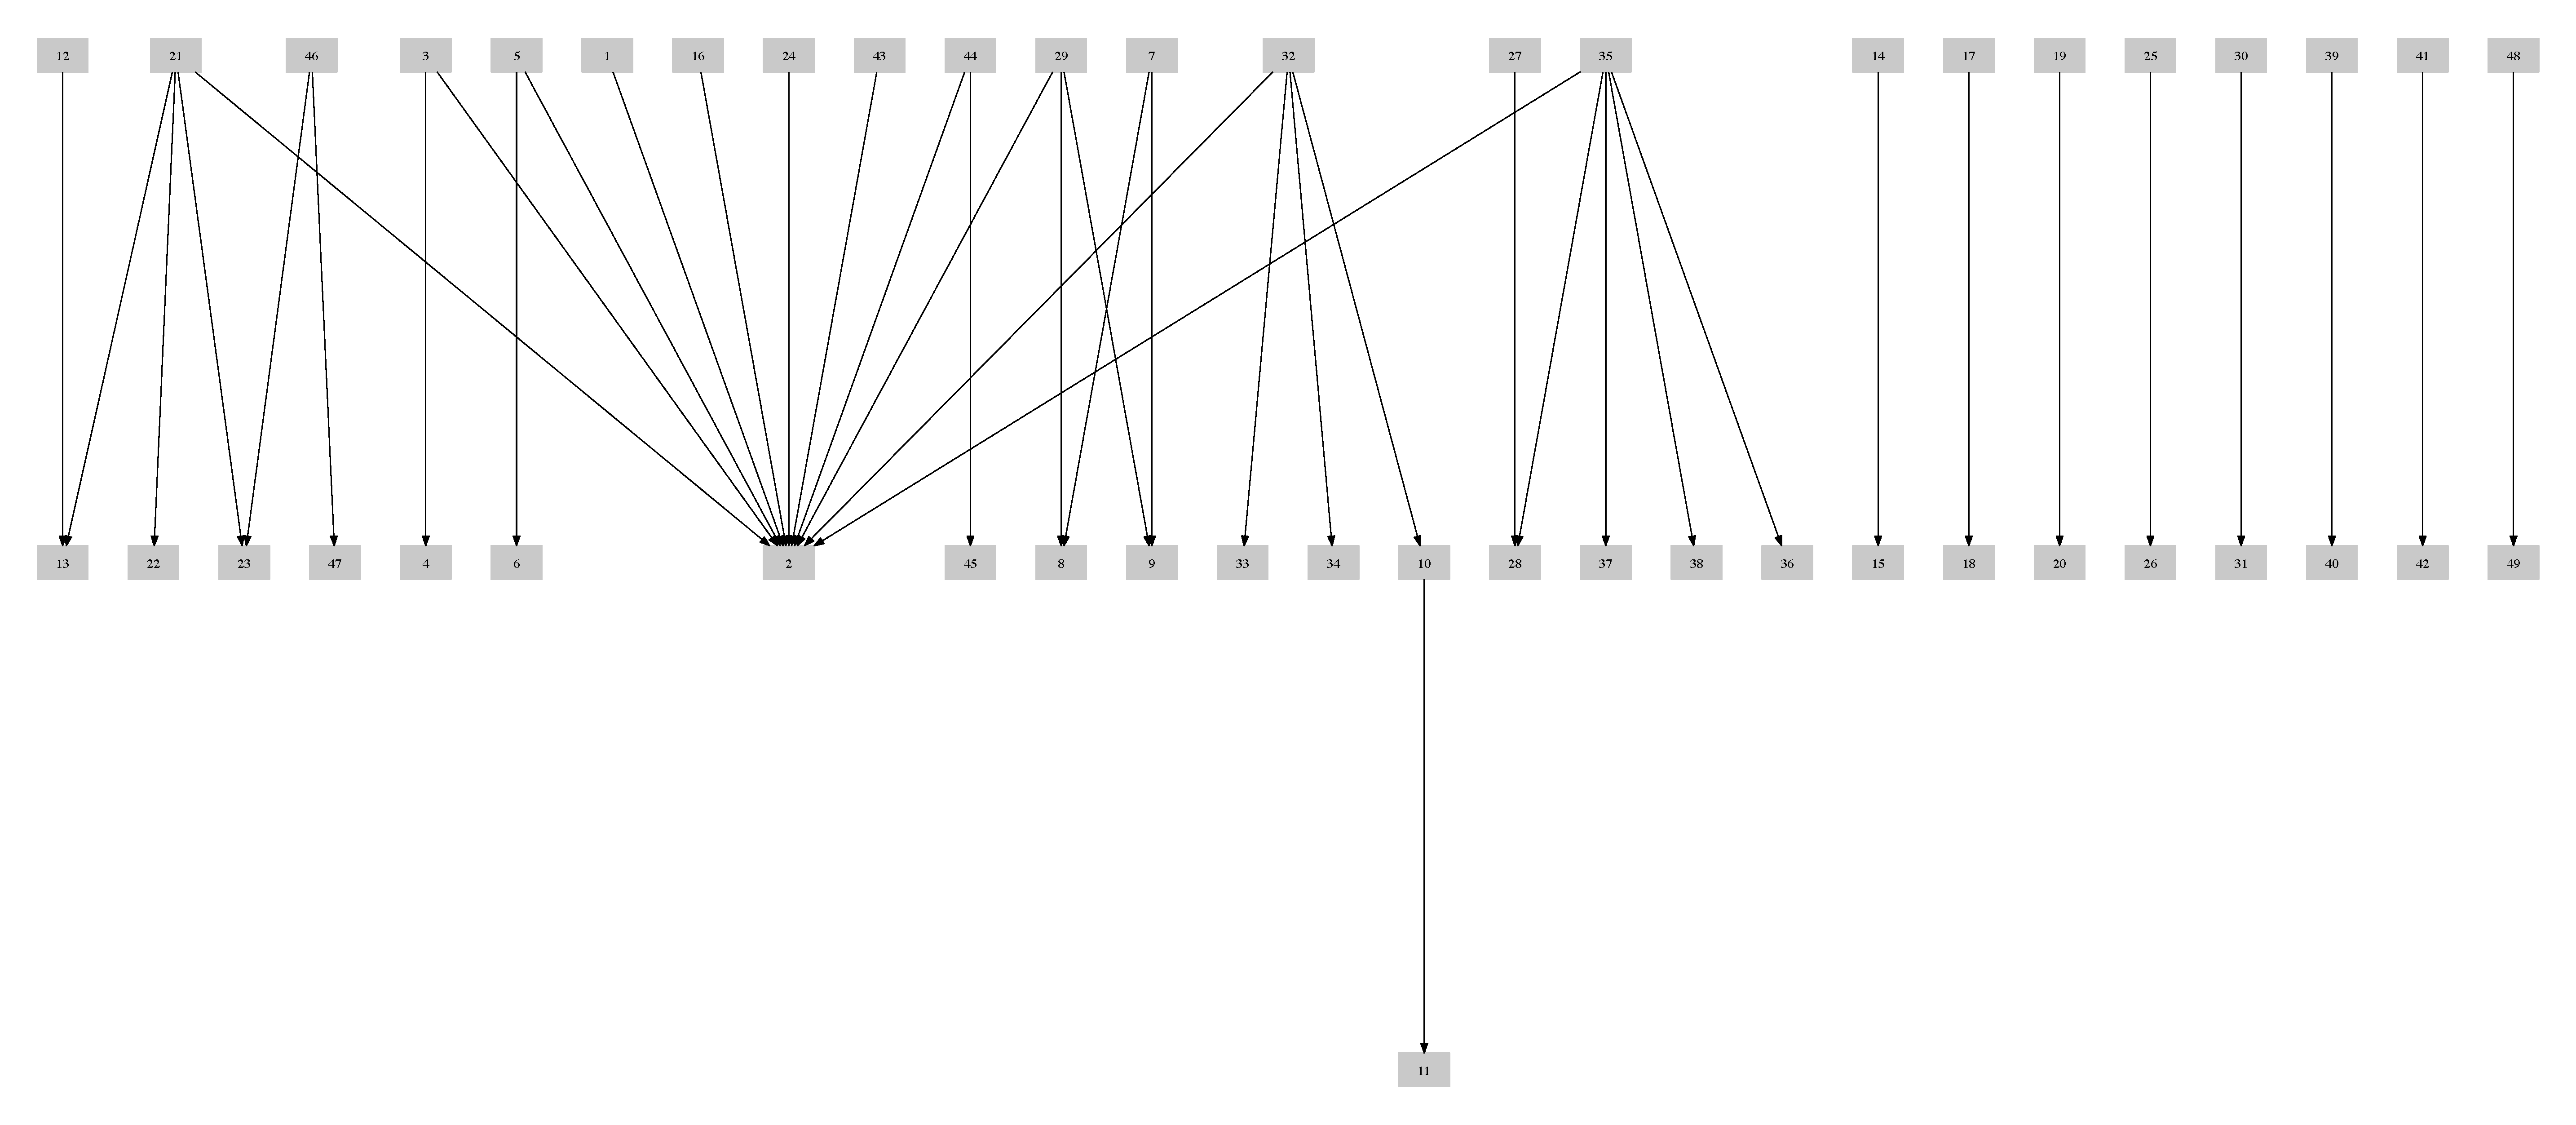
\includegraphics[angle=90, width=0.70\linewidth]{images/bazooka-masked-new-fixtures-bazooka-auto.pdf}
    \caption{Dependency graph generated from deployment configuration and executed with \textbf{automatic reverse service discovery} in the case study. The application identifiers are masked with incremented numbers.}
    \label{fig:deploy_env_auto}
  \end{figure}
\clearpage
}

To cross-validate these results, we manually determined the application identifiers for each value, taking the value and key name into account. The resulting graph can be seen in \autoref{fig:deploy_env_manual}.

\afterpage{%
\thispagestyle{empty}
  \begin{figure}[t]
    \vspace*{-3.5cm}
    \centering
    
\includegraphics[angle=90, width=0.50\linewidth]{images/bazooka-masked-new-fixtures-bazooka.pdf}
    \caption{Dependency graph generated from deployment configuration and executed with \textbf{manual reverse service discovery} in the case study. The application identifiers are masked with incremented numbers.}
    \label{fig:deploy_env_manual}
  \end{figure}
\clearpage
}

\subsubsection{Discussion}

We start the discussion by comparing the manually and automatically generated graphs with each other. The major difference between both are the sizes of the graphs. The automatically generated graph \ref{fig:deploy_env_auto} has 49 vertices and 41 edges, whereas the manual graph \ref{fig:deploy_env_manual} is about double as big with 88 vertices and 99 edges\footnote{Please note that between the different graphs, the numbering of the applications is not consistent. Thus, application ``1'' in one graph is not the same as application ``1'' in another graph. This is due to the mechanism of masking we used, which did not sync naming between the generation of the graphs.}. We attribute this difference to the fact that in the manual execution we have all reverse service discovery methods of the automated version available, plus are able to deal with edge cases manually. These included the following:
\begin{tdescription}
  \item[Decomposed URIs] We found 5 URIs that were decomposed into several configuration variables. One example for that is splitting the hostname and the portname into two variables, as visible in \autoref{list:bazookaconfexamplesplit}.
  \item[Incomplete URIs] 7 times we encountered URIs that did not fully denote a service. One example is the bazooka load balancer address as configuration value without the port number, as visible in \autoref{list:bazookaconfexamplesplit}, when only taking the ``bazookaLB'' variable into consideration.
  \item[Physical addressing not resolvable] We encountered several physical addresses, which were not automatically resolvable. We were able to resolve these manually with the help of the variable name as well as by logging into the respective machine and investigating the applied chef roles.
\end{tdescription}

Both graphs show the monolith of the architecture with a big number of incoming edges (vertex ``2'' with 11 incoming edges in the automated and vertex ``5'' with 13 incoming edges in the manual graph). We have seen the monolith to be mostly addressed via \emph{CNAMEs} with the application name. The database \emph{MySQL} (vertex ``2'') makes up for a significant share of the edges in the manually-created graph \autoref{fig:deploy_env_manual}. These are not represented in the automatically-addressed graph, since they addressed specific deploys of the application by IP address or physical machine name.

\begin{lstlisting}[caption=Example configuration of an application in Bazooka,label=list:bazookaconfexamplesplit]
{
  "bazookaLB": "bazooka-lb.internal.example.com",
  "threadedCommentsBazookaPort": 8485
}
\end{lstlisting}

% As long as there is no convention around how environment variables are structured, it will be hard to run this satisfyingly. Since the definition of these edge cases is subject to the creativity of the developers, we believe it will be impossible to handle all these edge cases completely.

\begin{table}
  \caption{Distribution of configuration cases for the dependency graph generated with manual reverse service discovery in \autoref{fig:deploy_env_manual}.}
  \label{tab:env_var_percentages}
  \begin{tabular}{ |l|l| }
    \hline
    Metric name & Value \\
    \hline
    Total number of configurations & 90 \\
    \hline
    Configurations without any variables & 17 \\
    Configurations with at least one variable & 73 \\
    \hline
    Configurations without any reverse service discoverable variables & 39 \\
    Configurations with at least one reverse service discoverable variable & 51 \\
    \hline
    Total number of dependencies discovered & 99 \\
    \hline
    Dependencies reverse service discoverable via Bazooka & 7 \\
    Dependencies reverse service discoverable via Glimpse & 1 \\
    Dependencies reverse service discoverable via CNAME & 65 \\
    Edge cases only service discoverable manually & 26 \\
    \hline
    CNAME discovered services directly mapping to an application name & 39 \\
    CNAME discovered services being deploys of the MySQL application & 22 \\
    CNAME discovered services being deploys of the RabbitMQ application & 4 \\
    \hline
  \end{tabular}
\end{table}

Table \ref{tab:env_var_percentages} shows more information about the distribution of the configuration. It can be seen that CNAME reverse service discovery makes up the majority of the discovered services. One of the assumption around CNAME discovery was that the \emph{name} is an application identifier. We found this assumption fulfilled in 60\% of cases, with the other cases denoting specific deploys of the \emph{MySQL} or \emph{RabbitMQ} applications (e.g. \lstinline{broker001.m.internal.example.com}).

In our investigations, we only found 1 case using the Glimpse service discovery. In that case, the ``product'' part of the URI did map the application identifier. Still, our method would benefit from either the convention that the ``product'' has to map the application identifier, or from another URI part that would include the application identifier. Among all methods of reverse service discovery, Glimpse proved to be the easiest to use. This is due to its well-defined URI format, which can be easily identifier via a regular expression, as well as the possibility to extract the identifiers without querying another system.

When comparing the graphs of this method with the earlier graph \nref{subsec:graph_manual_annotation}, we can see that the earlier graph has more vertices and edges (90 vertices/188 edges) than our graphs here (manual 88 vertices/99 edges and automated 49 vertices/41 edges). The earlier graph also has 7 hierarchy levels, whereas the graphs of this method only have 4 hierarchy levels. We attribute this to the fact that the graphs generated with the method here may only take applications into consideration which have been deployed with Bazooka, whereas the earlier graph may also take differently-deployed applications into consideration. It is to be noted that the comparability of the graphs is limited by the fact that there were several months between the generation of these graphs and more applications were created within this time period which are not present in earlier graph \nref{subsec:graph_manual_annotation}.

% Packet forwarding and domain aliasing make reverse service discovery more  complex. In our case study, one of these examples is the HAProxy load balancer by Bazooka, which

% precision/recall?
% Might have false-positives (if configuration has more, e.g. because legacy)
% Might have false-negatives (if not all service discovery is in configuration, which might happen)

One limitation during our investigation was the reverse service discovery for applications outside of the organizations scope like third-party services. Two practical examples we encountered in our investigation were the REST API of Twitter~\cite{twitterdev} as well as the Amazon S3 web services APIs~\cite{amazons3}. It would theoretically be possible to put these behind the internal service discovery mechanisms, but doing so is impractical, since it increases complexity without providing tangible direct benefits especially since the location of these external services is highly unlikely to change. Therefore we believe, these have to manually be mapped to application identifiers then.

To conclude, we have seen that the approach introduced in this chapter is \textbf{feasible}, since we were able to execute it in our case study. Its \textbf{correctness} and the degree of \textbf{automation} are influenced by how many of the requirements are met: Are all applications configured during deployment? Do all applications get their service dependency locations from that environment? Is it possible to obtain the configuration for the deploys? Is it possible to execute reverse service discovery for discovered service discovery locations? To structurally fulfill these requirements, we see deployment systems like Bazooka and service discovery systems like Glimpse as enabling factors.

\subsubsection{Future Work}

During the automated execution, we did not take the variable names into consideration. We did so during manual execution though. We found that variable names did not follow a convention. Still, they were useful in manually determining the service dependency application, even though this eventually meant ``guessing'' the actual application identifier. This could be improved by introducing a convention on environment variable names, which includes the application identifier. An example format is ``service\_{application\_identifier}''.

If the service locations are within the application's codebases and not in the environment, it might still be possible to execute this method. This assumes that we can extract the service locations from the codebase. We may then execute the same reverse service discovery mechanisms as explained before.

% Another method to handle service discovery is to do it within the application. An example is Zookeeper~\cite{zookeeper}, which is a distributed data store that was used as the basis for several service discovery systems in microservice architectures . Simplified, service discovery happens by accessing data in the zookeeper data store. Given we would be able. Instead of getting application dependencies from the environment, these might also exist within the application, for example if service discovery happens with Zookeeper. Then, would need to parse out of code all callsites for zookeeper and search for the key it is called with.

One of the edge cases we identified was physical addresses (e.g. IP addresses like  \emph{10.23.0.10} or physical domain names like \emph{app08.internal.example.com}). These do not hold service discovery information. If it is possible to connect to that address (e.g. via \emph{ssh}), investigations on the server could happen. Examples are investigating running processes (assuming a way to map processes to application identifiers) or applied chef roles (assuming a mapping from chef role to application). Both examples assume that a machine only has one application running.

\subsection{From network connections}
\label{subsec:from_network}

With this method we generate a dependency graph from the service dependencies of applications. We derive these service dependencies by observing network traffic and matching the source and destination processes to applications.

\subsubsection{Theory}

We assume that all application dependencies manifest themselves as network communication between the applications' processes. Thus if we detect network communication between two processes, we can derive that there is an application dependency between these applications.

To execute this method, we have to observe network communication. Assuming that communication is based on TCP/IP~\cite{internetprotocol}, we may take a TCP packet as atomic entity. A packet holds the information about the IP address and port number of the source and destination. If these can be mapped to their respective applications, we have determined the application dependency. If we are able to determine, which of the two communication parties started the communication, we can derive the direction of the application dependency, from source to destination.

Given all this information, the longer we observe the system, the more service dependencies may be collected. Each source or destination application becomes a vertex in the dependency graph and each observed service dependency becomes an edge.

\subsubsection{In the case study}

In our case study we executed this method in the context of applications deployed with Bazooka. We observed packets on the Bazooka application hosts. Each application host used a Linux distribution as operating system. We execute the packet observation using \emph{netstat}, which allows to display currently active network connections.

\begin{lstlisting}[caption=Sanitized example output from netstat. Schema is: local\_address foreign\_address process\_id/process\_name,label=list:netstatexample]
192.168.100.1:39998 192.168.100.3:1001 10411/application
192.168.100.1:2001 192.168.100.2:35019 20471/python
\end{lstlisting}

Listing \ref{list:netstatexample} shows an example output from netstat, which we filtered to include only the essential information. The IP address \emph{192.168.100.1} belongs to the machine where the capturing happened. The first line shows a connection that started from a local process to a remote service (\emph{outgoing connection}). The second line shows a connection that started from a remote process to a local service (\emph{incoming connection}). Next we will investigate for both cases, how to map the source and destination applications of the connection.

% A connection may either originate remotely (from another process to the machine currently under investigation) or locally (from the machine currently under investigation).

\paragraph{Source application} When a process opens a new network connection, it usually does so by using network sockets~\cite{sockets} \cite{SocketsProgramming}. A socket needs a local port, which it usually gets assigned by the operating system~\footnote{It is also possible for a process to bind to a specific local port. From our experience, this is common for server processes, since the location of their service has to be known to its clients. It is uncommon for client processes, since any port number works equally well, and a client process binding to a specific port number might get the problem of the port number already being occupied. Letting the operating system handle the concern alleviates the client process from the complexity of finding a free port number.}. If we now observe an incoming connection on a machine, there is no way to map that incoming port number to a process and/or application, since the port number has been assigned just for that connection.

Therefore we may only be able to map outgoing connections to application identifiers. Next we will describe that process in the context of the Bazooka application host. In the outgoing connection in \autoref{list:netstatexample} (first line) we can see that netstat returns a \emph{process\_id} and the \emph{process\_name}. The \emph{process\_name} does not reveal the application name, since processes have widely differing ways of being executed, resulting in no consistent mapping to application names. To do the mapping in our case study, we relied on implementation details of Bazooka: When a process is started on a Bazooka app host, it is executed within a Linux container (LXC~\cite{lxc}~\cite{lxcsuse}). These containers are isolated using Kernel Control Groups (cgroups~\cite{cgroups}). Via the proc virtual filesystem, it is possible to access the cgroup information for a specific process, which in turn contain the name of the container. Listing \ref{list:cgroupsexample} shows an example output of the cgroup information. Bazooka uses the following scheme for the container names: \newline \lstinline!{application}-{process}-{git-commit-sha}!. \newline We are able to extract the application identifier from that container name, and thus are able to map the source application for outgoing connections.

\begin{lstlisting}[caption=Cgroup information example from the proc virtual filesystem\, retrieved via \lstinline{cat /proc/20471/cgroup} in our case study,label=list:cgroupsexample]
1:perf\_event,net\_cls,freezer,devices,memory,cpuacct,cpu,cpuset:
  /lxc/threaded-comments-web-b3d7941-22160
\end{lstlisting}

\paragraph{Destination application} We have just shown that it is possible to obtain the source application identifier for \emph{outgoing connections}. Now we will show how to obtain the destination application identifier for such connections. The destination of a connection (or \emph{service location}) has the property that is has to be discoverable for the process wanting to connect to it. Commonly this discovery from a service discovery key to a service location is done via a service discovery mechanism. We are interested in doing this process in reverse, thus mapping from service location to the service discovery key and the to the application identifier. We call this process ``reverse service discovery'' and introduced several methods for it in the previous \nref{subsec:graphfromdeploymentconf}. The difference to the earlier execution and here is that we now only have IP addresses to work with. For example in the earlier listing \autoref{list:netstatexample}, the destination application has the IP address/port number pair of \lstinline{192.168.100.3:1001}. Next we will explain the execution for the Bazooka and Glimpse reverse service discovery:

\textbf{Bazooka} A service that is deployed with Bazooka is accessed via a port on the Bazooka load balancers. Given that we know the IP addresses of the Bazooka load balancer and have access to the HAProxy config file, we may map the application identifier the same way as introduced in earlier in \nref{subsec:graphfromdeploymentconf}.

\textbf{Glimpse} When we introduced reverse service discovery for Glimpse in earlier \nref{subsec:graphfromdeploymentconf}, we saw that the domain name format makes it possible to directly parse out the \emph{product} and therefore application identifier from a Glimpse service discovery domain.

To do the same in this method, we have to first map the IP address and port name to the Glimpse domain name. The Glimpse service discovery mechanism is based on BIND~\cite{bind}, which holds the information about the DNS mapping in a zonefile. Listing \ref{list:depgraphglimpse} shows an example excerpt from that zonefile. We can see that the product \emph{threaded-comments} has three instances. Each of these is identified with a physical domain name (e.g. \emph{app08.internal.example.com}) and a port number (e.g. \emph{1001}). Let's assume that we try to resolve the IP address \lstinline{192.168.100.3:1001} from earlier netstat example \autoref{list:netstatexample}. We first have to map the IP address to a physical domain name. We may do so with a reverse DNS lookup from address to domain name (as specified in RFC \cite{rfc1034} section 5.2.1.). Our example IP address \lstinline{192.168.100.3:1001} would then map to the physical domain name \emph{app08.internal.example.com}. We may use that physical domain name and the port number for a lookup in the zonefile, which leads to the Glimpse domain \emph{http.web.prod.threaded-comments.ca} and the product/application identifier \emph{threaded-comments}\footnote{It might be possible, to do reverse DNS lookup for SRV records, similar to reverse DNS lookups for IP addresses to domain names. Following the definition in RFC 6763 \cite{rfc6763} and our experience, we did not find a solution for that, other than the one introduced using the zonefile directly.}.

\begin{adjustwidth}{-0.9in}{-.8in}
    \begin{lstlisting}[caption=Glimpse zonefile example excerpt,label=list:depgraphglimpse]
      http.web.prod.threaded-comments.ca 5 IN SRV 0 0 1000 app08.internal.example.com
      http.web.prod.threaded-comments.ca 5 IN SRV 0 0 1001 app08.internal.example.com
      http.web.prod.threaded-comments.ca 5 IN SRV 0 0 5671 app78.internal.example.com
    \end{lstlisting}
\end{adjustwidth}

% \textbf{Semantic DNS CNAMEs} As already discussed in \nref{subsec:graphfromdeploymentconf}, engineers may assign CNAME domains to certain machines. These names may then be used as application identifiers during reverse service discovery. To discover the semantic CNAME for an IP address, we may use a reverse DNS lookup (as specified in RFC \cite{rfc1034} section 5.2.1.).

In our case study we executed the connection gathering and analysis with both reverse service discovery methods on March 14 2014. Next we will describe the process we used:
\begin{titemize}
  \item We executed the connection observations sequentially on all Bazooka application server. On each server, we executed netstat 50 successive times with a 5ms delay between the executions. We then collected the cgroup records for all processes on each application host\footnote{ This is based on the assumption that processes do exist for an extended amount of time, but at least between doing the connection observation and retrieving the mapping between process ID and cgroup. We found that to be true, with process IDs only changing when a process was restarted (for example when it crashed or a new deployment was done) or when it was stopped for administrative reasons (for example when the number of running process instances per deploy is decreased)}.
  \item We collected the zonefile from a BIND server by Glimpse\footnote{All instances of BIND in Glimpse used the same zonefile.}.
  \item We collected the HAProxy configuration file from a Bazooka load balancer\footnote{All instances of the Bazooka load balancers used the same HAProxy configuration file.}.
  \item We manually determined the addresses of all Bazooka load balancers.
  \item To analyze the data, we took each collected network connection and tried to map that to an application dependency with the methods explained above.
\end{titemize}

As a result of the investigation, we were able to derive 260 connection pairs between processes running on a Bazooka app host and a remote host. Of these, we resolved 9 application dependencies via the Bazooka load balancers and 2 application dependencies via Glimpse. Figure \ref{fig:graph_from_network} shows the resulting graph.

\begin{figure}[h]
  \begin{center}
    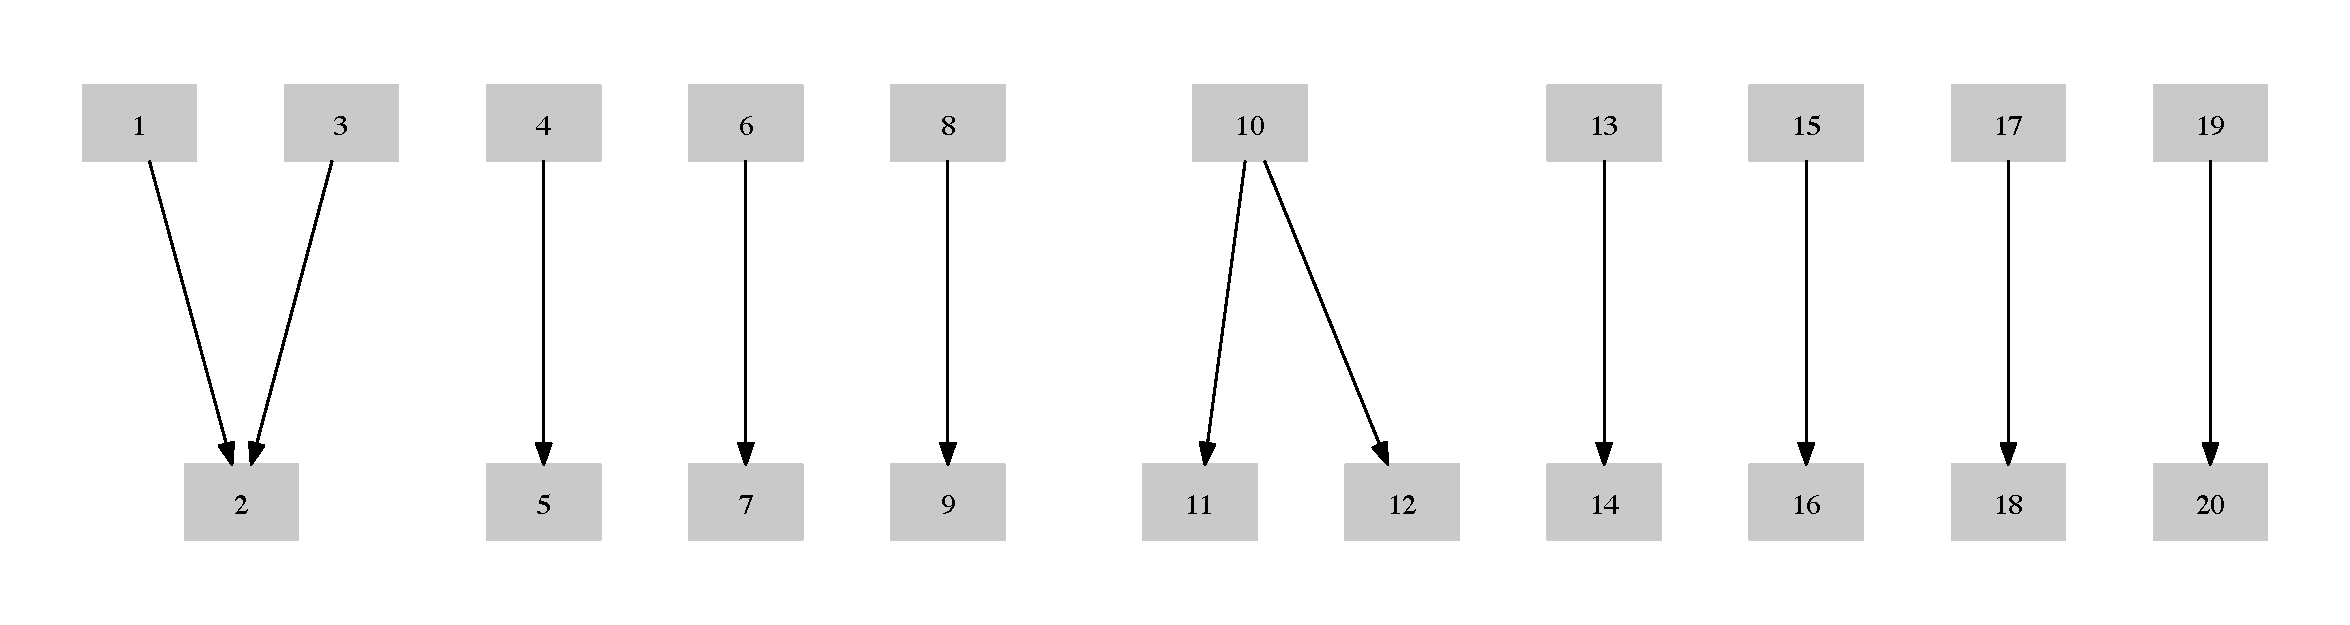
\includegraphics[width=1\textwidth]{images/from-network-connections.pdf}
  \end{center}
  \caption{Dependency graph: Graph from network connections, resulting from execution in the case study. Application names are masked.}
  \label{fig:graph_from_network}
\end{figure}

\subsubsection{Discussion}

Given the resulting graph in \ref{fig:graph_from_network} we can see that only few applications and dependencies were identified. Also these are not well-connected. We conclude that at least the graph we created in the case study is not a satisfying representation of the actual state of the architecture we investigated.

A major problem with this method is identifying the source application of a connection. In our case study investigation, we used an implementation detail of Bazooka to collect the information. This appears to be a brittle approach since there are no guarantees that this implementation detail might not change in future versions of Bazooka. It also is not possible to use the approach when other systems than Bazooka are used for deployment.

An easier problem to solve was mapping the destination application of a connection, given that we assume mechanisms for reverse service discovery to exist. During our investigations we were able to only resolve a small subset of destination applications (11 from 260). We attribute these to a low adoption of Glimpse. We also did not take ``Semantic DNS CNAMEs'' into consideration, which in earlier \nref{subsec:graphfromdeploymentconf} made up for a significant share of services.

% As impeding factors we see a low adoption of Glimpse in our case study, as well as the fact that applications deployed on Bazooka typically mostly have application dependencies on backing applications, which in turn are stateful and thus not deployed with Bazooka. In our case study, these applications are not part of service discovery, but usually identified via their physical hostnames. We think, that it is possible to have all deploys under service discovery, which then would then also allow inverse service discovery for all destination application. The exception might be applications that are outside of the organization's boundary, for example external REST APIs.

In our case study implementation, we probed for current connections at regular intervals. Therefore, we are not able to detect connections that did not happen at the times of probing. Examples might be application dependencies that have low traffic or only have traffic during certain times. The probability of detecting all connections increases if measurements are done over a longer time period.

% Given this would measure for a very long time, depending on the rate of change between application dependencies, it might capture too many dependencies. For example if application A has a dependency to database B, but then changes that to a dependency to database C, if the measurement was executed over the length of the change, the dependencies to both databases would be visible in the graph.

We measured connections on all Bazooka application hosts. Depending on the number of hosts, this might be a substantial effort, with regards to orchestration of the measurement and impact on the running system. Also, the measuring itself might create big data volumes to be analyzed. These might be handled by analyzing the connections immediately and aggregating the results on the machine.

One problem we did not investigate are networking mechanisms like network address translation or proxy servers. Since these effectively hide the true origin IP address, they might impede on the possibility for reverse service discovery.

To conclude, we have shown that this method is \textbf{feasible}, even though in our case study we only detected a subset of the application dependencies. The  \textbf{correctness} of the method depends on the mechanism to detect connections, as well the mechanisms for mapping source and destination IP addresses and ports reliably to application identifiers. In our case study, we have shown that it is possible to execute the method in an \textbf{automated} way.

\subsubsection{Future Work}

% We have found the mapping of source applications to be a major problem of the method. Next, we will introduce some options for future investigations:
%
% A more structured way would be to implement the functionality with the Bazooka Repository Manager, as a well-defined API. Holds true for
%
% Different ways of mapping source applications. A suggestion would be Port ranges? Then possible to do

To measure connections, another option to investigate is measuring on the network directly. Networking equipment like switches do allow to the monitoring of connections and packets \cite{Hogg}. The problem here is deriving the source application, which in our case study involved knowledge that only exists on the applications hosts, thus making network capturing infeasible. Instead of the network, communication might also happen via other media. An example is the ``Service Bus'' in SOA as explained in \cite{enterpriseSOA} section 4.3.4.

We also see three options for future work regarding ``reverse service discovery'':
\begin{titemize}
  \item In earlier \ref{subsec:graphfromdeploymentconf}, we introduced the ``reverse service discovery'' method \emph{Semantic DNS CNAMEs}. We did not use this method in the case study execution here but believe that it might improve the results significantly.
  \item More work can be done in exploring how to map IP addresses to application names. For example Chef might be used, in the same way as already explained in earlier \ref{subsec:graphfromdeploymentconf}.
  \item Packet inspection could be used to identify source applications. For example, the packet content could be annotated with the source application identifier. A practical implementation could be using the HTTP protocol with a custom header holding that information. This is similar to the way tracing frameworks work, which we will introduce in the following section \ref{section:graph_future_work}.
\end{titemize}

\section{Discussion}

We introduced four methods for generating an application dependency graph from a deployed microservice architecture.
\begin{tdescription}
  \item[\ncref{subsec:graph_manual_annotation}] We found this method to be the most complete and correct method. We showed that it is feasible to execute this method within an organization. By its nature, this method is only semi-automated. The gathering of annotations and graph generation may be automated. The creation and maintenance of dependency information is manual.
This impedes on the feasibility of the method (due to lack of knowledge with the executing people) and the correctness (due to lack of knowledge with the executing people, differing willingness of people in the organization to create annotations, continuous effort to adapt annotations to change in architecture).
  \item[\ncref{subsec:from_smi}] We found the assumptions of this method not to be fulfilled in our case study. To correctly identify internal application dependencies, these would have to be deliberately encapsulated, which appears to be a significant change to existing codebases. Also, the problem of mapping module names to application dependencies seems to only be solvable by manual mappings. We conclude that this method might be feasible, but would demand significant effort to change existing structures.
  \item[\ncref{subsec:graphfromdeploymentconf}] We found this method to be feasible and potentially providing correct results. The execution of the method can be automated. In the case study execution, we found that only some service dependencies could be mapped to application identifiers, since reverse service discovery was not always possible. Also we only investigated deploys done with the \emph{Bazooka} deployment system, thus we did not capture all deployed applications.
  \item[\ncref{subsec:from_network}] We found this method to be feasible within our case study. Problematic was mapping the applications, which limited the method in our investigations.
\end{tdescription}

Since in our case study only \ncref{subsec:graph_manual_annotation} gave us a complete picture of the architecture, we will continue using the dependency graph we constructed from our case study with that method in the following chapters.

We did an informal qualitative evaluation of that graph with engineers of the case study company. A common reaction was to search for the applications the particular engineers were concerned with in their daily work. From there they analyzed and discussed incoming and outgoing edges. It occurred that existing edges were surprising to engineers and showed unexpected dependencies. Circular dependencies were a topic of concern for engineers, which were identified and discussed with the help of the dependency graph. A common concern for the dependency graph was as to which extent it represents the currently deployed architecture. We also learned that other engineers in the past tried to create similar graphs manually. They never created a meaningfully complete graph of all applications, but rather either only looked for a small subset, usually from the perspective of one application or they made a high-level architecture diagram which did not follow a consistent or holistic entity model. Other architecture overviews we encountered were data flow diagrams and request flow diagrams. Both were usually based on actual deploys of applications and only featured a limited subset of the architecture.

We believe that \ncref{subsec:graphfromdeploymentconf} and \ncref{subsec:from_network} are feasible automated ways to generate application dependency graphs and might be fruitful for future work. They both make assumptions towards the infrastructure tooling, especially with regards to reverse service discovery. It is to be investigated, how these can be satisfied without compromising other requirements, like low system complexity or scalability.

A problem with all methods was to distinguish applications that are currently deployed in the production deployment environment. We proposed criteria for manually filtering applications in manual creation (among them excluding infrastructure, deprecated and prototype applications). The same criteria were then used for manually filtering applications in the other methods as well. With all methods we hoped to find ways of running them highly-automated, but eventually did not succeed in doing so. All methods needed manual intervention at some point, for example when filtering for applications and deploys that are part of the production deployment environment.

If microservice architecture continue to grow in popularity, we expect ``programmable infrastructure'' to become more prevalent. We see programmable infrastructure as the attribute of systems to enable the planning, creation, maintenance and monitoring of an architecture. These systems will then also allow programmable interaction, which in turn allows for more sophisticated analysis of the architecture, just as we have executed them in this chapter.

% PaaS is awesome
% In our investigations, we have seen ``programmable infrastructure'' tools (e.g. Bazooka). We see that it is beneficial to our cause to be able to have standardized ways for
% PaaS approaches and virtualization of infrastructure are likely to help lots. "Programmable infrastructure" with standardized access to all parts of the infrastructure. Currently it is "detective work" in deriving infromation from many different sources. The topology, location and the format of these data sources change over time, making human interaction needed.

% Going forward, we use the manual annotation version

% Why are we on level of application? Assumption that it is useful to argue here, since applications are natural level of abstraction from a programmers perspective. Also discussion ownership (both source code and deploy) often happens on application level. This leads to allocation of engineering time happening on the same level.

\section{Future work}
\label{section:graph_future_work}

% central overview (soa service repository, enterprise service bus
% Did AOL publish something about their infrastructure?

A method worth investigate more is deriving service dependencies from within source code. We touched onto one option for this in the ``Future work'' section of \nref{subsec:graphfromdeploymentconf}, where we proposed extracting service locations or service discovery keys from the source code. Another option would be to annotate dependencies to services in the code e.g. with a comment.

Tracing frameworks like Dapper \cite{dapper} or Zipkin \cite{zipkin} allow for collecting information on how requests travel through a system. This assumes a request/response style communication originating in one part of the system (usually the interface to the user). Each of these request gets an identifier, which is carried through the architecture when more requests are made to subsystems. This tracing information is then collected and made available for analysis. Even though initially meant for performance monitoring, tracing would also allow to extract service dependencies.

% In our work, we only investigated application dependencies that manifest via network communication. Future work could investigate other forms of application dependencies. Examples are message queues or shared data storage.

An interesting angle for future work is using a finer granularity when discovering dependencies. In our work we used applications and application dependencies. A more fine-grained approach would be by using processes. An even more detailed approach would be splitting applications or processes into functionalities and modeling dependencies between these. For example, if a service provides several HTTP resource locations, each of these could be seen as a functionality, to which other application functionality might have dependencies. Each resource location in turn would be a functionality with own dependencies. This would allow for more sophisticated dependency modeling, which in turn could also lead to new angles in dependency modeling.

\section{Summary}

The goal of this chapter was to evaluate ways of creating a dependency graph from a deployed and running microservice architecture. A dependency graph is a directed graph with applications as vertices and service dependencies as directed edges from service consumer to service provider. We proposed four novel methods for creating dependency graphs, all of which we executed in the context of our case study in a real and deployed microservice architecture. We then evaluated each method after the aspects feasibility, correctness and automation.

Of the four methods, \ref{subsec:graph_manual_annotation} manually annotating service dependencies and semi-automatically collecting these for constructing the dependency graph was the most viable option, since it provided the most complete view on the deployed architecture. The graph we constructed from our case study with that method is visible in \autoref{fig:manual_annotation_whole}.

% \item[] {\small\ref{subsec:graph_manual_annotation} \ncref{subsec:graph_manual_annotation}}
% \item[] {\small\ref{subsec:from_smi} \ncref{subsec:from_smi}}
% \item[] {\small\ref{subsec:graphfromdeploymentconf} \ncref{subsec:graphfromdeploymentconf}}
% \item[] {\small\ref{subsec:from_network} \ncref{subsec:from_network}}
%
